\chapter{Symbols and Rituals}

In 1994, we had the official inauguration of Harnham's Dhamma Hall. For
the two years prior to that, a great deal of time and effort had gone
into the construction and finishing of the building. Nothing seemed to
happen very fast in Northumberland, and gradually I was getting used to
that. By character I can be a bit speedy, so this more modest mode of
operating was good for me.

Shortly after Tan Ajahn Chah had passed away, two local sculptors who
were friends of the monastery, Ken and Jenny, humbly asked if, on behalf
of the extended lay community, they might express gratitude and respect
to our late Teacher by carving a stone \emph{stupa} and presenting it to
the monastery. Their generous offering was gladly accepted. This was
just one example of several local artisans who significantly contributed
to this emerging spiritual sanctuary.

My memory is that carving the stupa did not take too long. What was
trickier was the installation. We agreed that it would be a nice idea to
position the approximately two-and-a-half-metre-high stupa in the middle
of a small pond. Of course the pond would have to be watertight and Ken
and Jenny went to great lengths to ensure it was well-built. When the
\emph{stupa} arrived at the monastery, it was delivered on the opposite
side of the Dhamma Hall from where it was going to be installed as part
of a Tan Ajahn Chah memorial garden. Transporting that half metric ton
of stone on rollers, across the new wooden floor of the Dhamma Hall was
quite a feat. The really delicate stage, though, came when this
immensely heavy object had to be raised and suspended from a tripod over
the plinth in the middle of the pond, and then, ever-so-gently, lowered
down onto ice-cubes, so there would be enough manoeuvrability to slide
it into its final position. Any sudden impact on the base could have
broken the seal on the pond. Thank you, Ken and Jenny, for such an
exquisitely beautiful act of devotion. It is indeed a fitting gesture of
gratitude to our teacher. Now, approximately twenty-five years later,
although the pond has been filled in and the stone of the \emph{stupa}
is partially coated in moss, the surrounding fern garden is kept tidy,
and every few years a devout Burmese layman comes with gold leaf and
reguilds the finial.

Ken and Jenny were likewise responsible for crafting the `moon-stone'
that sits at the entrance to the Dhamma Hall, also for the front door
handles and the handsome \emph{Dhammacakka} sculpture in the vestibule.
It was a lot of fun visiting the workshops of these craftspeople and
discussing the details of the various projects. The traditional
`moon-stone', which is often found at entrance ways to Sri Lankan
temples, is usually a highly stylised piece compared to the modest,
understated version we have. It seems that the original symbolic
significance of the `moon-stone' was the cyclic nature of \emph{samsara}\cite{sandakada}.

In the case of Harnham's entranceway, on the corners of the stone slabs
surrounding the moon-stone, there were placed four brass etchings of the
`divine messengers\cite{divine}' -- old age, sickness, death and a wandering
monk. They were inset there as symbolic reminders of how it is often the
suffering of life that inspires us to turn away from a path of heedless
distraction and enter upon the spiritual journey. We so easily become
intoxicated by momentary happiness, unaware that there is the
possibility of awakening to an unshakeable form of happiness. Suffering
can sober us up and reveal the possibility of an altogether different
approach to life.

The bronze handles on the front doors to the Dhamma Hall depict, on the
right-hand side, a dragon, symbolising \emph{hiri} and \emph{ottappa}\cite{hiri};
on the left hand side there is a representation of the world: \emph{hiri} and
\emph{ottappa} are watching over the world. The Buddha referred to
\emph{hiri} and ottappa, as \emph{lokapala}, `protectors of the world'.
The decision to locate depictions of these important Dhamma principles
on the front doors was a way of saying that, before we can enter the
spiritual sanctuary, our heart must be imbued with a wholesome sense of
shame and a fear of doing that which is unskilful.

The word `shame' has heavy connotations for many Westerners because of
the pain of having been taught when we were young that we are all
sinners. When such spiritual instruction is not imparted wisely, it
fails in its intent to instil an appreciation for virtue; instead it
just makes people feel bad about themselves. The Buddha called these two
aspects of virtue -- \emph{hiri} and \emph{ottappa} -- protectors,
because that is what they do; they protect our psychological world and
conduce to inner balance, as well as having a wholesome influence on the
outer world. It doesn't take a lot of thought to appreciate how, when we
act heedlessly and shamelessly, there are unpleasant consequences, for
ourselves and for the world in which we live.

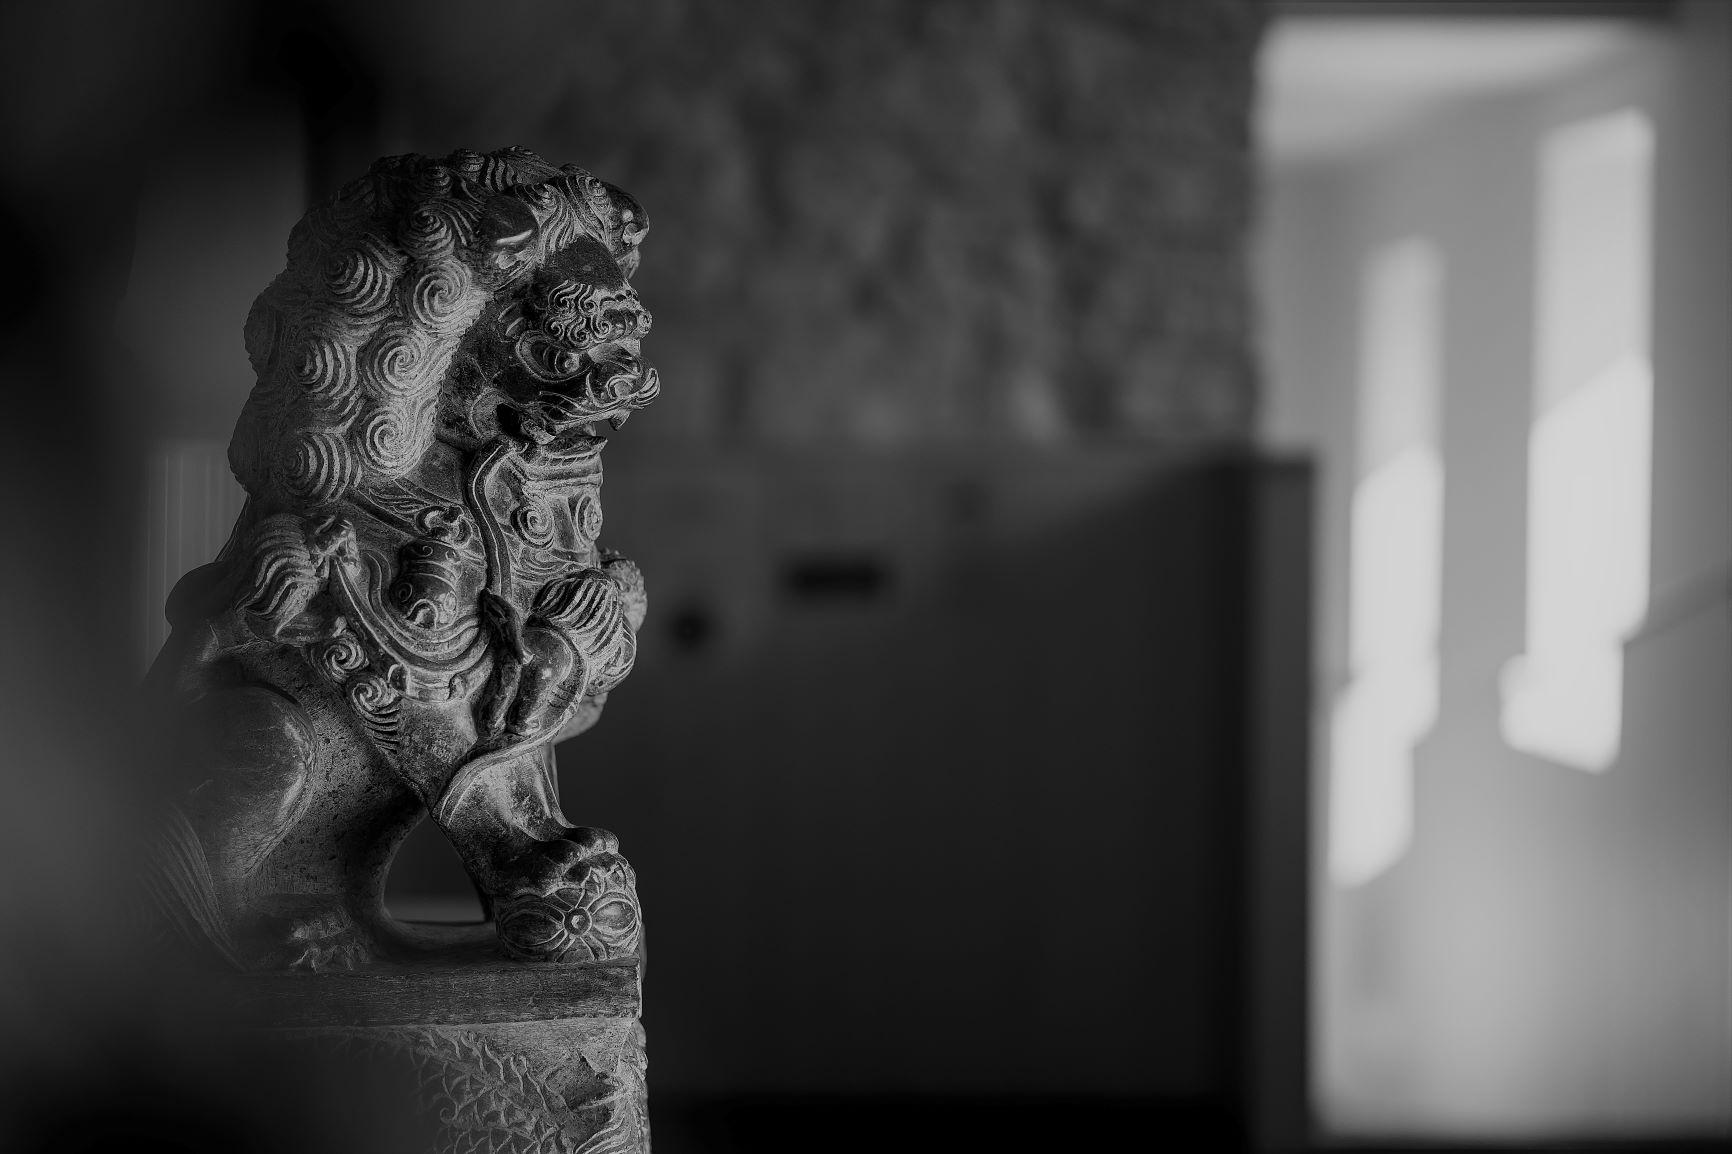
\includegraphics[width=\linewidth]{image9.jpeg}

Once visitors have entered the vestibule of the Dhamma Hall, they are
immediately confronted with two large black stone lions. These weren't
carved locally, but were purchased by my friend, Mark Overton, while he
was working as a doctor in Beijing, and shipped to Newcastle. Two
supporters of our monastery who lived in Glasgow, Sena and Aruni,
sponsored them. I wanted them placed at the entrance like that, to
symbolically test the resolve of those who entered. Perhaps we have been
inspired by suffering to seek an alternative to the casual pursuits that
we have hitherto followed, and have enough moral confidence to take the
first steps, but we need to know that our resolve will be tested,
probably over and over again. We need to learn to be daring and
courageous.

Above the two lions is a carving of the Dhamma wheel, the symbol for the
Buddha's teachings. For the last two thousand years, since Alexander the
Great from Greece\cite{greco} forayed into what is now Afghanistan, we have had Buddha
images which serve to inspire followers of this path of practice.
However, the Buddha himself recommended using the wheel as a symbolic
object of devotion. The \emph{Dhammacakkappavattana Sutta}, his first
recorded discourse, means \emph{Setting the Wheel of Dhamma in Motion}\cite{cakka}.
There were other objects that
he endorsed, such as the Bodhi Tree and a Dhamma Seat, but it is perhaps
the wheel that has become best known.

It was important to me that we engaged local artisans in the work of
designing the Dhamma Hall. Yes, we are a branch monastery of Wat Pah
Pong in North East Thailand, and many of our visitors are from that part
of the world. There are also many who come from just a few miles away.
Someone once reported to me a comment made by His Holiness the Dalai
Lama, when he was asked what he thought about Tibetan Buddhism in
America. Apparently he said, `Rather too Tibetan.' I wanted our friends
from Thailand, Laos, Cambodia, Malaysia, Myanmar and Sri Lanka to all
feel at home in our monastery, but I also wanted the Europeans who
joined us for evening meditation or on retreat, to feel at ease. This
was all part of integrating Buddhism into this culture at this time.

Once you enter the Dhamma Hall itself, you will see in the centre of the
oak floor, a very large rug. Theo and Val, who lived in a small town
called Coldstream, just across the border into Scotland, had started
visiting the monastery. They worked as weavers and were part of a Craft
Centre on The Hirsel Estate\cite{hirsel}. When I discussed with Theo the
idea of having a large rug with a Dhammacakka woven into it, he was
enthusiastic. It would be no small undertaking for a cottage craftsman,
but he was keen. The meditation group in Leeds, called Dhammapala,
offered to sponsor the wool for the project. A great many rolls of yarn
would be required. Theo's first introduction to Buddhism had been via
the Tibetan tradition and he tried hard to persuade me that the rug
should be designed in bright primary colours. My preference was to have
the inside of the hall feel connected with the outside. After some
mild-mannered debating, Theo acquiesced, and a massive amount of moss
coloured yarn was ordered.

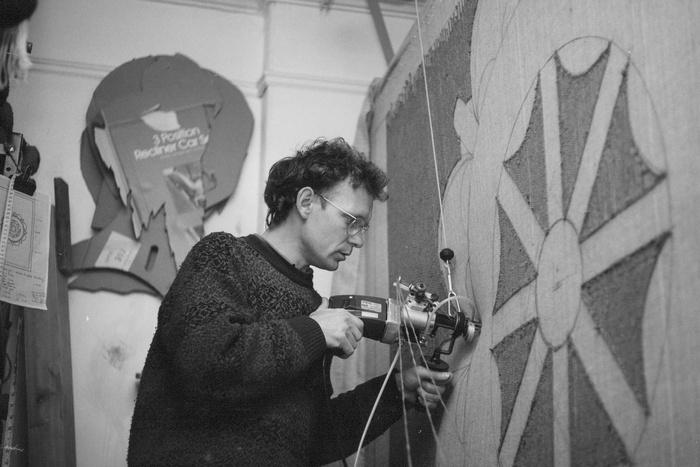
\includegraphics[width=\linewidth]{image10.jpeg}

Once the bulk of the work on the rug had been completed, there was still
the task of refining the carving of the wheel design into it; it wasn't
a woven rug, it was tufted. This would require laying the rug out in a
large, clean, empty space. Theo and Val lived in the Lodge (Gatehouse)
of the Hirsel and didn't have a room big enough. At that time, the
14th Earl of Home\cite{earl} (pronounced Hewm), Sir Alec Douglas-Home, an ex-Prime
Minister of Great Britain, was living in the main house with his
daughter Caroline. Caroline was very helpful in allowing Theo to make
use of a large room in the main house that, at the time, was not
occupied. The result of all the effort is beautiful. I expect the rug
will continue to grace our Dhamma Hall for many years to come.

When Jody Higgs, one of the monastery's trustees, retired, she wanted to
mark the occasion with a special offering. We discussed it and agreed
that it would be good to engage one of Scotland's skilled potters to
produce a raku\cite{raku} style pot to use as the main incense dish
on the shrine. What
she produced looks just right. It sits on the `just right' puja table
constructed by a local cabinet maker, who also built the Dhamma Seat.

Another piece that was at least partially produced locally is the wall
mural. Traditionally, in Thai temples the mural on the wall directly
opposite the main Buddha image and shrine is a depiction of the
Buddha-to-be sitting under the bodhi tree, conquering the hordes of
\emph{Mara}. Khun Pang Chinasai, a Thai artist known for his skill and
experience in traditional temple painting, was commissioned by a
supporter from Guildford to do the work. Since we didn't have the right
sort of wall on which to paint, and perhaps for other reasons, Khun Pang
decided to produce the painting on a huge canvas that would later be
fixed to the wall. This also meant he could get started while he was in
London. When it had reached a stage of being ready for the more refined
details, he brought the canvas up to Harnham and completed it on-site. I
don't know exactly how long it took him, but it required great
dedication and focus. He had a practice of getting up very early in the
morning to sit meditation and then start on the painting. It was
impressive to watch, for example, when it came to the parts of the mural
which were in gold, the precision with which he applied the gold leaf.
The refinement of detail was extraordinary.

In keeping with ancient tradition, the mural tells a story. At the
centre is the bodhi tree under which the Buddha-to-be
(\emph{Bodhisattva}) is seated -- composed, reflective, resolute. His
right hand is reaching down and touching the earth, which indicates that
he is asking \emph{Mae Thorani} to bear witness to his right to seek
liberation. There is a depiction of \emph{Mae Thorani} beneath the
Bodhisattva; she is wringing water from her hair, symbolizing all the
accumulated wholesome potential (\emph{puñña}) that the Bodhisattva had
generated over many lifetimes in pursuit of freedom. On the right-hand
side of the mural, the hordes of \emph{Mara} can be seen in warring
mode, hurling spears and threats at the Bodhisattva. As the spears and
arrows get near to where he is seated, the force and purity of his
resolve transforms them into flowers. On the left-hand side of the mural
the hordes can be seen with their hands raised in \emph{añjali} asking
for forgiveness, having recognised their mistake. Towards the top of the
painting there are depictions of celestial beings (\emph{devas}) who are
intentionally keeping their distance.

For someone brought up in a traditional Theravada Buddhist culture, it
would be normal to relate to activities in these non-visible realms of
existence as if they were literally true. Others, who have been reared
in a more secular materialistic culture, would probably find it hard to
believe literally in the existence of such dimensions. Whether one
believes literally or reads the depictions figuratively, the story still
conveys a powerfully relevant message. The Bodhisattva under the bodhi
tree represents the heart that is unshakeably resolved to awakening from
unawareness. The hordes of \emph{Mara} are the myriad impulses that have
the power to distract and intimidate anyone who dares to aspire for
awakening. The celestial beings hiding away up in the clouds attempting
to escape the unpleasantness, are all of our clever ideas about
practice; when it comes to truly confronting the consequences of having
indulged for so long in unawareness, they abandon us. It takes much more
than bright ideas to transform unawareness into wisdom and compassion.

When Khun Pang had finished his work on the mural, members of the local
Thai community flew His Excellency the Royal Thai Ambassador up from
London to participate in a celebration of this magnificent work.

On the occasion of the Thai Ambassador's visit, Ajahn Sumedho was also
with us, and this marked the inauguration of the Dhamma Hall. In that
month of August 1994, I also conducted our first \emph{pabbajja} (novice
precepts ceremony). Anagarika Axel requested the Ten Precepts of a
samanera and was given the name Revato.

